% =====================================================================
% Clase -- Geometría 6° -- Trimestre I -- Semana 05
% Sesión 004 (lun 28 sep., 13:40, 50 min)
% Tema: Ángulos entre rectas
% Subtema: Adyacentes y opuestos por el vértice; bisectriz
% Hilo conductor del trimestre I: «La geometría del fútbol»
% Tema 2 de la guía: Ángulos entre rectas (tema:angulosrectas)
% Material del docente (no se entrega a los estudiantes).
% =====================================================================
\documentclass[11pt]{article}
\makeatletter\def\input@path{{../../../../../plantillas/estilo/}}\makeatother
\usepackage{mmcantillo}
\guiadelestudiante{../../guia-didactica/guia-periodo-I-angulos-poligonos}

\tipodocumento{Clase}
\asignatura{Geometría}
\titulo{Semana 5: lo que pasa donde se cruzan dos líneas}
\grado{6°}
\periodo{I}

% DBA: matematicas grado 6 · DBA 5 — Utiliza y explica diferentes estrategias (desarrollo de
% la forma, cubrimiento con cuadrados) e instrumentos (regla, compás) para calcular ángulos.
% DBA 6 — Representa y construye formas bidimensionales a partir de las medidas de sus lados
% y ángulos. Evidencias de esta sesión: hallar medidas de ángulos a partir de relaciones
% (adyacentes y opuestos por el vértice) sin medir con transportador, y construir la bisectriz
% como recurso para dividir un ángulo en dos iguales.

\begin{document}

\encabezado*

\begin{center}
{\renewcommand{\arraystretch}{1.3}
\begin{tabularx}{\linewidth}{@{}l l l X l@{}}
  \toprule
  \textbf{Sesión} & \textbf{Fecha} & \textbf{Min} & \textbf{Subtema} & \textbf{Entregables}\\
  \midrule
  004 & lun 28 sep., 13:40 & 50 & Adyacentes, opuestos por el vértice y bisectriz
      & Quiz (5 pts) y tarea (5 pts)\\
  \bottomrule
\end{tabularx}}
\end{center}

Hasta ahora medimos ángulos sueltos con el transportador. Hoy los ángulos dejan de estar
sueltos: cuando dos rectas se cruzan aparecen cuatro a la vez, y conocer uno basta para saber
los otros tres. Es el primer razonamiento de la asignatura en que \emph{se deduce} una medida
en vez de medirla. Siguiendo el hilo, la línea de banda y la línea de medio campo del estadio
son el cruce de rectas que tenemos a la mano. Referencia: \refguia{tema:angulosrectas}.

% ---------------------------------------------------------------------
\seccion{Sesión 004 — lunes 28 de septiembre · 13:40 · 50 min}

\textbf{Objetivo.} Reconocer ángulos adyacentes y opuestos por el vértice, deducir con ellos
las tres medidas que faltan cuando se conoce una, y trazar la bisectriz de un ángulo con regla
y compás.

\textbf{Materiales.} Regla, compás y transportador (cada estudiante); tablero; la guía.

\begin{center}
{\renewcommand{\arraystretch}{1.3}
\begin{tabularx}{\linewidth}{@{}l l X@{}}
  \toprule
  \textbf{Momento} & \textbf{Min} & \textbf{Actividad}\\
  \midrule
  Enganche & 0--6 & Dos rectas cruzadas en el tablero, sin números. Se mide \emph{uno} solo de
    los cuatro ángulos: $47^\circ$. «¿Alguien se atreve a decir los otros tres antes de que los
    midamos?» Se anotan las apuestas y se miden. Salen $133^\circ$, $47^\circ$ y $133^\circ$.\\
  Los nombres & 6--18 & \textbf{Adyacentes}: comparten el vértice y un lado; juntos forman una
    línea recta, así que suman $180^\circ$. \textbf{Opuestos por el vértice}: no comparten
    ningún lado, están «en diagonal». Escribir la deducción completa en el tablero: si
    $\alpha + \gamma = 180^\circ$ y $\beta + \gamma = 180^\circ$, entonces $\alpha = \beta$.
    Subrayar que eso no se midió: se \emph{demostró}, y por eso vale para cualquier medida.\\
  Práctica rápida & 18--28 & Cuatro cruces dibujados en el tablero, cada uno con un ángulo
    dado ($30^\circ$, $90^\circ$, $115^\circ$, $152^\circ$). En el cuaderno, los otros tres de
    cada uno. El de $90^\circ$ deja ver algo: si uno es recto, los cuatro lo son.\\
  Bisectriz & 28--42 & Definición: la semirrecta que parte un ángulo en dos iguales. Se traza
    con compás, paso a paso y todos a la vez: (1) con centro en el vértice, un arco que corte
    los dos lados; (2) con centro en cada corte y la misma abertura, dos arcos que se crucen;
    (3) la semirrecta del vértice a ese cruce. Comprobar con el transportador que las dos
    mitades quedaron iguales.\\
  Quiz & 42--50 & Quiz individual (5 puntos). Al recogerlo se deja la tarea.\\
  \bottomrule
\end{tabularx}}
\end{center}

\textbf{Figura para el tablero: cuatro ángulos, un solo dato.}

\begin{center}
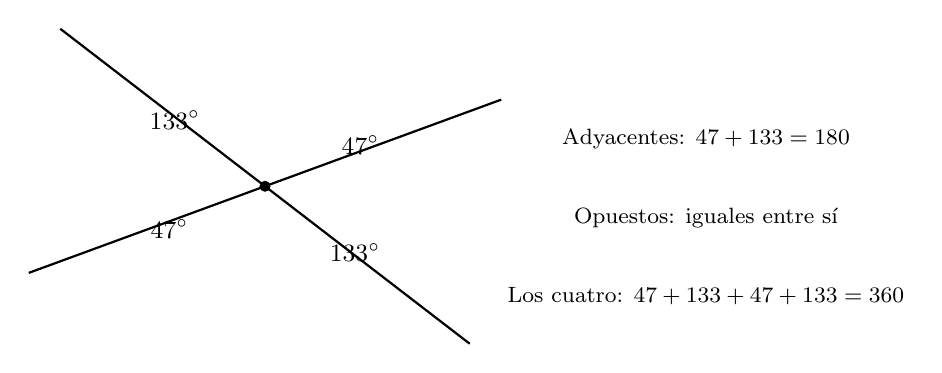
\begin{tikzpicture}[scale=1.0, every node/.style={font=\small}]
  \draw[thick] (-3,-1.1) -- (3,1.1);
  \draw[thick] (-2.6,2) -- (2.6,-2);
  \coordinate (O) at (0,0);
  \fill (O) circle (2pt);
  \node[above right] at (0.85,0.28) {$47^\circ$};
  \node[above left]  at (-0.7,0.6)  {$133^\circ$};
  \node[below left]  at (-0.85,-0.3){$47^\circ$};
  \node[below right] at (0.7,-0.6)  {$133^\circ$};
  \node[align=left, font=\footnotesize] at (5.6,0.6)
    {Adyacentes: $47 + 133 = 180$};
  \node[align=left, font=\footnotesize] at (5.6,-0.4)
    {Opuestos: iguales entre sí};
  \node[align=left, font=\footnotesize] at (5.6,-1.4)
    {Los cuatro: $47+133+47+133 = 360$};
\end{tikzpicture}
\end{center}

\begin{nota}
\textbf{Dónde suele trabarse.} En confundir «opuestos por el vértice» con «los de enfrente»
dicho a ojo, y terminar emparejando dos adyacentes. El criterio seguro es el de los lados: si
comparten un lado son adyacentes; si no comparten ninguno, son opuestos. Conviene hacerles
señalar los lados con el dedo antes de decidir.
\end{nota}

\begin{nota}
\textbf{La comprobación de los $360^\circ$.} Vale la pena dejarla instalada como costumbre: si
los cuatro ángulos no suman $360^\circ$, hay un error en alguna parte, y se ve sin rehacer
nada. Es la misma idea que usarán toda la secundaria para revisar su propio trabajo.
\end{nota}

\begin{nota}
\textbf{Si el compás falla.} No todos traen compás en buen estado. Alternativa para trazar la
bisectriz: doblar el papel de modo que un lado del ángulo caiga exactamente sobre el otro; el
pliegue \emph{es} la bisectriz. Sirve además para que vean por qué funciona.
\end{nota}

\end{document}
